\documentclass[1p]{elsarticle_modified}
%\bibliographystyle{elsarticle-num}

%\usepackage[colorlinks]{hyperref}
%\usepackage{abbrmath_seonhwa} %\Abb, \Ascr, \Acal ,\Abf, \Afrak
\usepackage{amsfonts}
\usepackage{amssymb}
\usepackage{amsmath}
\usepackage{amsthm}
\usepackage{scalefnt}
\usepackage{amsbsy}
\usepackage{kotex}
\usepackage{caption}
\usepackage{subfig}
\usepackage{color}
\usepackage{graphicx}
\usepackage{xcolor} %% white, black, red, green, blue, cyan, magenta, yellow
\usepackage{float}
\usepackage{setspace}
\usepackage{hyperref}

\usepackage{tikz}
\usetikzlibrary{arrows}

\usepackage{multirow}
\usepackage{array} % fixed length table
\usepackage{hhline}

%%%%%%%%%%%%%%%%%%%%%
\makeatletter
\renewcommand*\env@matrix[1][\arraystretch]{%
	\edef\arraystretch{#1}%
	\hskip -\arraycolsep
	\let\@ifnextchar\new@ifnextchar
	\array{*\c@MaxMatrixCols c}}
\makeatother %https://tex.stackexchange.com/questions/14071/how-can-i-increase-the-line-spacing-in-a-matrix
%%%%%%%%%%%%%%%

\usepackage[normalem]{ulem}

\newcommand{\msout}[1]{\ifmmode\text{\sout{\ensuremath{#1}}}\else\sout{#1}\fi}
%SOURCE: \msout is \stkout macro in https://tex.stackexchange.com/questions/20609/strikeout-in-math-mode

\newcommand{\cancel}[1]{
	\ifmmode
	{\color{red}\msout{#1}}
	\else
	{\color{red}\sout{#1}}
	\fi
}

\newcommand{\add}[1]{
	{\color{blue}\uwave{#1}}
}

\newcommand{\replace}[2]{
	\ifmmode
	{\color{red}\msout{#1}}{\color{blue}\uwave{#2}}
	\else
	{\color{red}\sout{#1}}{\color{blue}\uwave{#2}}
	\fi
}

\newcommand{\Sol}{\mathcal{S}} %segment
\newcommand{\D}{D} %diagram
\newcommand{\A}{\mathcal{A}} %arc


%%%%%%%%%%%%%%%%%%%%%%%%%%%%%5 test

\def\sl{\operatorname{\textup{SL}}(2,\Cbb)}
\def\psl{\operatorname{\textup{PSL}}(2,\Cbb)}
\def\quan{\mkern 1mu \triangleright \mkern 1mu}

\theoremstyle{definition}
\newtheorem{thm}{Theorem}[section]
\newtheorem{prop}[thm]{Proposition}
\newtheorem{lem}[thm]{Lemma}
\newtheorem{ques}[thm]{Question}
\newtheorem{cor}[thm]{Corollary}
\newtheorem{defn}[thm]{Definition}
\newtheorem{exam}[thm]{Example}
\newtheorem{rmk}[thm]{Remark}
\newtheorem{alg}[thm]{Algorithm}

\newcommand{\I}{\sqrt{-1}}
\begin{document}

%\begin{frontmatter}
%
%\title{Boundary parabolic representations of knots up to 8 crossings}
%
%%% Group authors per affiliation:
%\author{Yunhi Cho} 
%\address{Department of Mathematics, University of Seoul, Seoul, Korea}
%\ead{yhcho@uos.ac.kr}
%
%
%\author{Seonhwa Kim} %\fnref{s_kim}}
%\address{Center for Geometry and Physics, Institute for Basic Science, Pohang, 37673, Korea}
%\ead{ryeona17@ibs.re.kr}
%
%\author{Hyuk Kim}
%\address{Department of Mathematical Sciences, Seoul National University, Seoul 08826, Korea}
%\ead{hyukkim@snu.ac.kr}
%
%\author{Seokbeom Yoon}
%\address{Department of Mathematical Sciences, Seoul National University, Seoul, 08826,  Korea}
%\ead{sbyoon15@snu.ac.kr}
%
%\begin{abstract}
%We find all boundary parabolic representation of knots up to 8 crossings.
%
%\end{abstract}
%\begin{keyword}
%    \MSC[2010] 57M25 
%\end{keyword}
%
%\end{frontmatter}

%\linenumbers
%\tableofcontents
%
\newcommand\colored[1]{\textcolor{white}{\rule[-0.35ex]{0.8em}{1.4ex}}\kern-0.8em\color{red} #1}%
%\newcommand\colored[1]{\textcolor{white}{ #1}\kern-2.17ex	\textcolor{white}{ #1}\kern-1.81ex	\textcolor{white}{ #1}\kern-2.15ex\color{red}#1	}

{\Large $\underline{12a_{0058}~(K12a_{0058})}$}

\setlength{\tabcolsep}{10pt}
\renewcommand{\arraystretch}{1.6}
\vspace{1cm}\begin{tabular}{m{100pt}>{\centering\arraybackslash}m{274pt}}
\multirow{5}{120pt}{
	\centering
	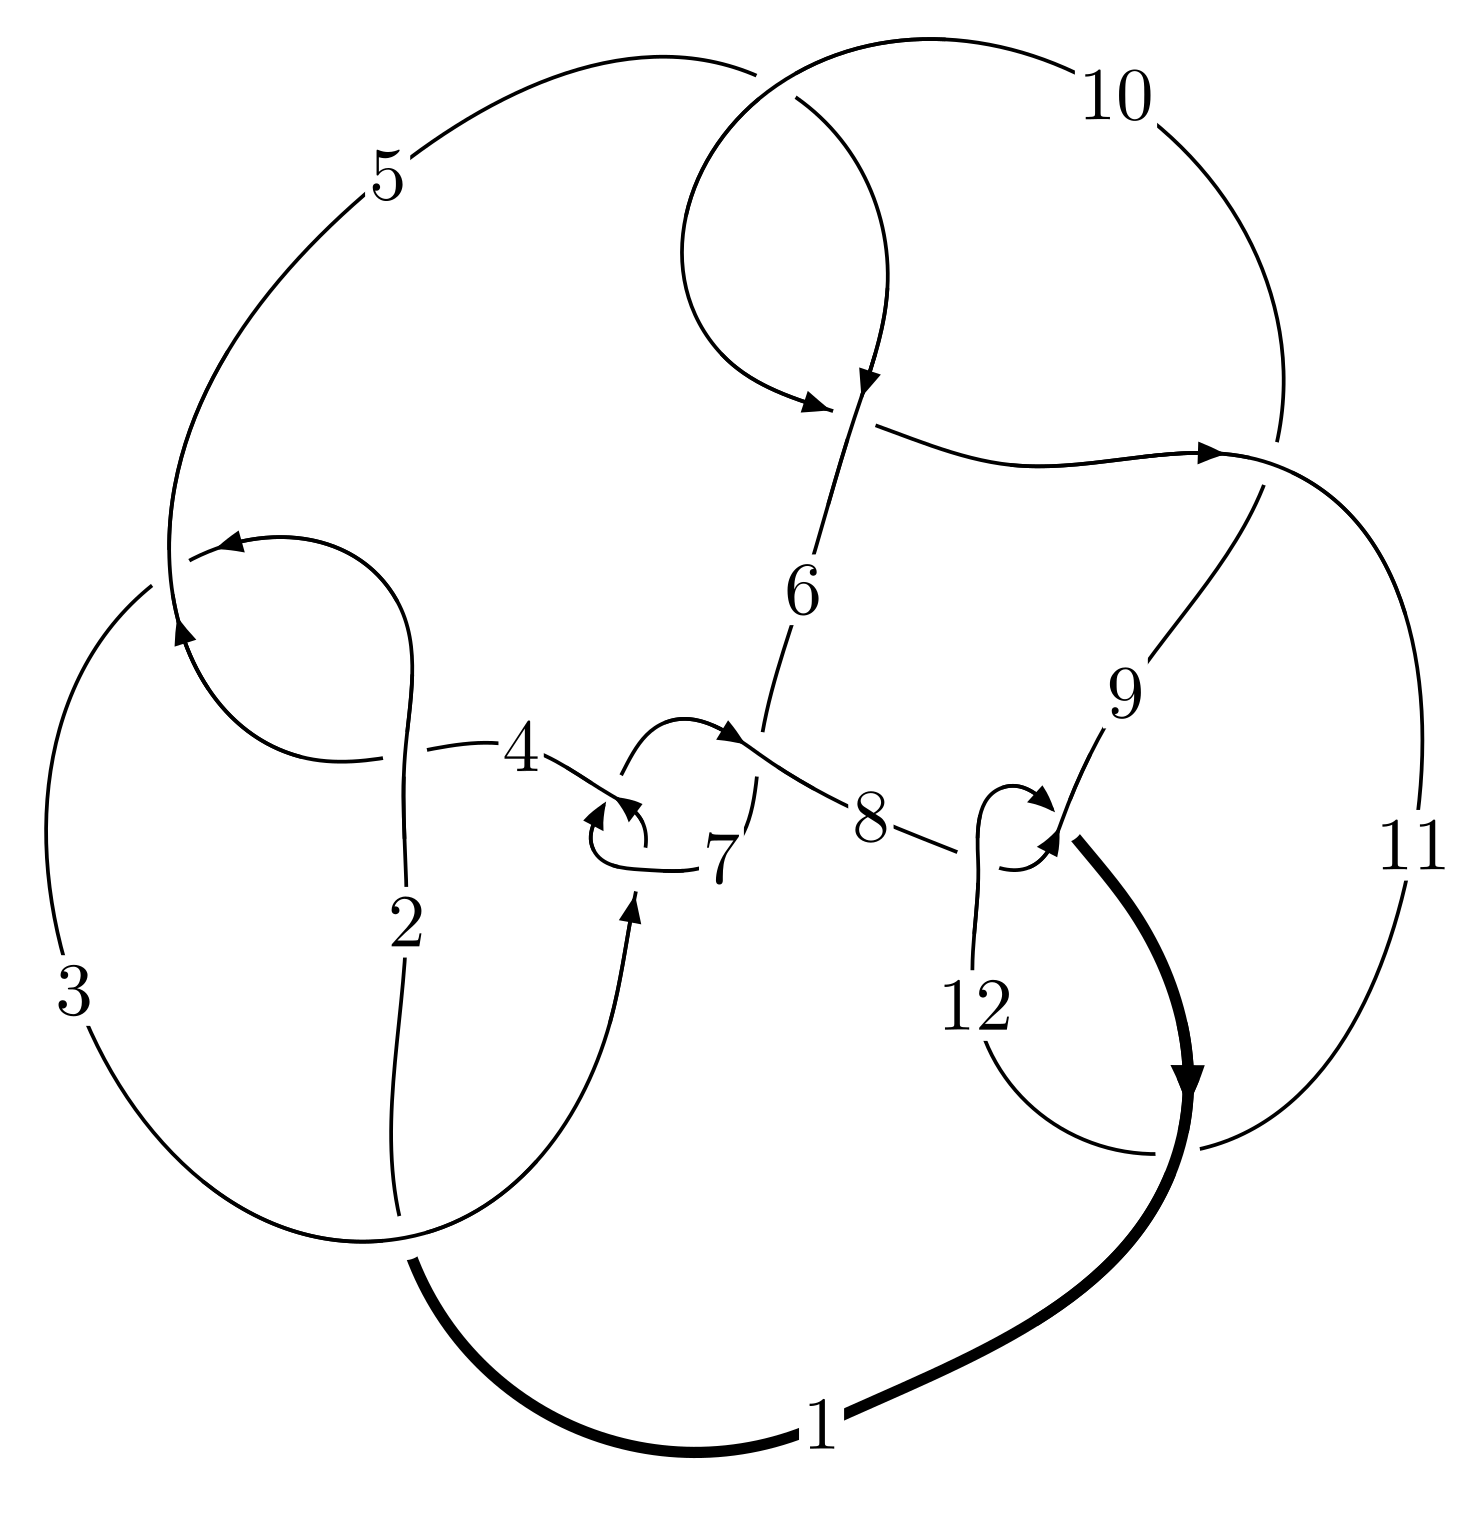
\includegraphics[width=112pt]{../../../GIT/diagram.site/Diagrams/png/859_12a_0058.png}\\
\ \ \ A knot diagram\footnotemark}&
\allowdisplaybreaks
\textbf{Linearized knot diagam} \\
\cline{2-2}
 &
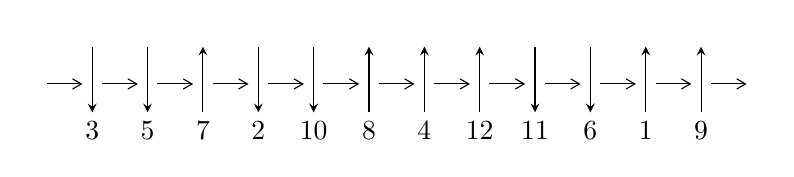
\begin{tikzpicture}[x=20pt, y=17pt]
	% nodes
	\node (C0) at (0, 0) {};
	\node (C1) at (1, 0) {};
	\node (C1U) at (1, +1) {};
	\node (C1D) at (1, -1) {3};

	\node (C2) at (2, 0) {};
	\node (C2U) at (2, +1) {};
	\node (C2D) at (2, -1) {5};

	\node (C3) at (3, 0) {};
	\node (C3U) at (3, +1) {};
	\node (C3D) at (3, -1) {7};

	\node (C4) at (4, 0) {};
	\node (C4U) at (4, +1) {};
	\node (C4D) at (4, -1) {2};

	\node (C5) at (5, 0) {};
	\node (C5U) at (5, +1) {};
	\node (C5D) at (5, -1) {10};

	\node (C6) at (6, 0) {};
	\node (C6U) at (6, +1) {};
	\node (C6D) at (6, -1) {8};

	\node (C7) at (7, 0) {};
	\node (C7U) at (7, +1) {};
	\node (C7D) at (7, -1) {4};

	\node (C8) at (8, 0) {};
	\node (C8U) at (8, +1) {};
	\node (C8D) at (8, -1) {12};

	\node (C9) at (9, 0) {};
	\node (C9U) at (9, +1) {};
	\node (C9D) at (9, -1) {11};

	\node (C10) at (10, 0) {};
	\node (C10U) at (10, +1) {};
	\node (C10D) at (10, -1) {6};

	\node (C11) at (11, 0) {};
	\node (C11U) at (11, +1) {};
	\node (C11D) at (11, -1) {1};

	\node (C12) at (12, 0) {};
	\node (C12U) at (12, +1) {};
	\node (C12D) at (12, -1) {9};
	\node (C13) at (13, 0) {};

	% arrows
	\draw[->,>={angle 60}]
	(C0) edge (C1) (C1) edge (C2) (C2) edge (C3) (C3) edge (C4) (C4) edge (C5) (C5) edge (C6) (C6) edge (C7) (C7) edge (C8) (C8) edge (C9) (C9) edge (C10) (C10) edge (C11) (C11) edge (C12) (C12) edge (C13) ;	\draw[->,>=stealth]
	(C1U) edge (C1D) (C2U) edge (C2D) (C3D) edge (C3U) (C4U) edge (C4D) (C5U) edge (C5D) (C6D) edge (C6U) (C7D) edge (C7U) (C8D) edge (C8U) (C9U) edge (C9D) (C10U) edge (C10D) (C11D) edge (C11U) (C12D) edge (C12U) ;
	\end{tikzpicture} \\
\hhline{~~} \\& 
\textbf{Solving Sequence} \\ \cline{2-2} 
 &
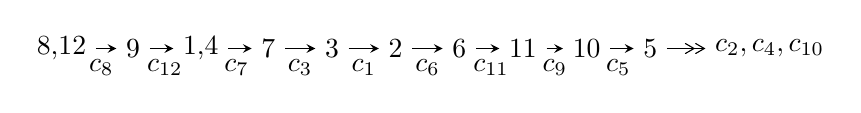
\begin{tikzpicture}[x=23pt, y=7pt]
	% node
	\node (A0) at (-1/8, 0) {8,12};
	\node (A1) at (1, 0) {9};
	\node (A2) at (33/16, 0) {1,4};
	\node (A3) at (25/8, 0) {7};
	\node (A4) at (33/8, 0) {3};
	\node (A5) at (41/8, 0) {2};
	\node (A6) at (49/8, 0) {6};
	\node (A7) at (57/8, 0) {11};
	\node (A8) at (65/8, 0) {10};
	\node (A9) at (73/8, 0) {5};
	\node (C1) at (1/2, -1) {$c_{8}$};
	\node (C2) at (3/2, -1) {$c_{12}$};
	\node (C3) at (21/8, -1) {$c_{7}$};
	\node (C4) at (29/8, -1) {$c_{3}$};
	\node (C5) at (37/8, -1) {$c_{1}$};
	\node (C6) at (45/8, -1) {$c_{6}$};
	\node (C7) at (53/8, -1) {$c_{11}$};
	\node (C8) at (61/8, -1) {$c_{9}$};
	\node (C9) at (69/8, -1) {$c_{5}$};
	\node (A10) at (11, 0) {$c_{2},c_{4},c_{10}$};

	% edge
	\draw[->,>=stealth]	
	(A0) edge (A1) (A1) edge (A2) (A2) edge (A3) (A3) edge (A4) (A4) edge (A5) (A5) edge (A6) (A6) edge (A7) (A7) edge (A8) (A8) edge (A9) ;
	\draw[->>,>={angle 60}]	
	(A9) edge (A10);
\end{tikzpicture} \\ 

\end{tabular} \\

\footnotetext{
The image of knot diagram is generated by the software ``\textbf{Draw programme}" developed by Andrew Bartholomew(\url{http://www.layer8.co.uk/maths/draw/index.htm\#Running-draw}), where we modified some parts for our purpose(\url{https://github.com/CATsTAILs/LinksPainter}).
}\phantom \\ \newline 
\centering \textbf{Ideals for irreducible components\footnotemark of $X_{\text{par}}$} 
 
\begin{align*}
I^u_{1}&=\langle 
9.29564\times10^{38} u^{113}-6.51435\times10^{39} u^{112}+\cdots+2.60710\times10^{37} b-7.95403\times10^{38},\\
\phantom{I^u_{1}}&\phantom{= \langle  }-7.77552\times10^{38} u^{113}+6.00866\times10^{39} u^{112}+\cdots+2.60710\times10^{37} a+1.51982\times10^{39},\\
\phantom{I^u_{1}}&\phantom{= \langle  }u^{114}-8 u^{113}+\cdots-8 u+1\rangle \\
I^u_{2}&=\langle 
- a^5+a^4-2 a^2+b+a+1,\;a^6- a^5+2 a^3- a^2- a+1,\;u+1\rangle \\
I^u_{3}&=\langle 
b,\;u^3- u^2+a+1,\;u^6- u^5- u^4+2 u^3- u+1\rangle \\
\\
\end{align*}
\raggedright * 3 irreducible components of $\dim_{\mathbb{C}}=0$, with total 126 representations.\\
\footnotetext{All coefficients of polynomials are rational numbers. But the coefficients are sometimes approximated in decimal forms when there is not enough margin.}
\newpage
\renewcommand{\arraystretch}{1}
\centering \section*{I. $I^u_{1}= \langle 9.30\times10^{38} u^{113}-6.51\times10^{39} u^{112}+\cdots+2.61\times10^{37} b-7.95\times10^{38},\;-7.78\times10^{38} u^{113}+6.01\times10^{39} u^{112}+\cdots+2.61\times10^{37} a+1.52\times10^{39},\;u^{114}-8 u^{113}+\cdots-8 u+1 \rangle$}
\flushleft \textbf{(i) Arc colorings}\\
\begin{tabular}{m{7pt} m{180pt} m{7pt} m{180pt} }
\flushright $a_{8}=$&$\begin{pmatrix}1\\0\end{pmatrix}$ \\
\flushright $a_{12}=$&$\begin{pmatrix}0\\u\end{pmatrix}$ \\
\flushright $a_{9}=$&$\begin{pmatrix}1\\- u^2\end{pmatrix}$ \\
\flushright $a_{1}=$&$\begin{pmatrix}u\\- u^3+u\end{pmatrix}$ \\
\flushright $a_{4}=$&$\begin{pmatrix}29.8244 u^{113}-230.473 u^{112}+\cdots+370.662 u-58.2952\\-35.6550 u^{113}+249.869 u^{112}+\cdots-225.591 u+30.5091\end{pmatrix}$ \\
\flushright $a_{7}=$&$\begin{pmatrix}13.8635 u^{113}-108.058 u^{112}+\cdots+140.743 u-18.9405\\19.6275 u^{113}-116.224 u^{112}+\cdots-51.7393 u+12.4153\end{pmatrix}$ \\
\flushright $a_{3}=$&$\begin{pmatrix}0.00677419 u^{113}-12.2366 u^{112}+\cdots+63.7165 u-10.4574\\13.4820 u^{113}-101.626 u^{112}+\cdots+177.807 u-30.9627\end{pmatrix}$ \\
\flushright $a_{2}=$&$\begin{pmatrix}-1.32665 u^{113}+18.2745 u^{112}+\cdots-88.4400 u+16.7723\\16.0974 u^{113}-99.1423 u^{112}+\cdots-25.0868 u+8.27723\end{pmatrix}$ \\
\flushright $a_{6}=$&$\begin{pmatrix}-5.76401 u^{113}+8.16502 u^{112}+\cdots+192.482 u-31.3558\\19.6275 u^{113}-116.224 u^{112}+\cdots-51.7393 u+12.4153\end{pmatrix}$ \\
\flushright $a_{11}=$&$\begin{pmatrix}- u^3\\u^5- u^3+u\end{pmatrix}$ \\
\flushright $a_{10}=$&$\begin{pmatrix}u^6- u^4+1\\- u^8+2 u^6-2 u^4\end{pmatrix}$ \\
\flushright $a_{5}=$&$\begin{pmatrix}9.56619 u^{113}-88.7065 u^{112}+\cdots+213.455 u-33.7200\\25.0853 u^{113}-158.460 u^{112}+\cdots+15.0149 u+1.68646\end{pmatrix}$\\&\end{tabular}
\flushleft \textbf{(ii) Obstruction class $= -1$}\\~\\
\flushleft \textbf{(iii) Cusp Shapes $= -164.292 u^{113}+1202.16 u^{112}+\cdots-1572.01 u+235.414$}\\~\\
\newpage\renewcommand{\arraystretch}{1}
\flushleft \textbf{(iv) u-Polynomials at the component}\newline \\
\begin{tabular}{m{50pt}|m{274pt}}
Crossings & \hspace{64pt}u-Polynomials at each crossing \\
\hline $$\begin{aligned}c_{1}\end{aligned}$$&$\begin{aligned}
&u^{114}+60 u^{113}+\cdots+8 u+1
\end{aligned}$\\
\hline $$\begin{aligned}c_{2},c_{4}\end{aligned}$$&$\begin{aligned}
&u^{114}-8 u^{113}+\cdots-8 u+1
\end{aligned}$\\
\hline $$\begin{aligned}c_{3},c_{7}\end{aligned}$$&$\begin{aligned}
&u^{114}-2 u^{113}+\cdots+128 u+64
\end{aligned}$\\
\hline $$\begin{aligned}c_{5},c_{10}\end{aligned}$$&$\begin{aligned}
&u^{114}+2 u^{113}+\cdots-128 u+64
\end{aligned}$\\
\hline $$\begin{aligned}c_{6}\end{aligned}$$&$\begin{aligned}
&u^{114}-42 u^{113}+\cdots-90112 u+4096
\end{aligned}$\\
\hline $$\begin{aligned}c_{8},c_{12}\end{aligned}$$&$\begin{aligned}
&u^{114}+8 u^{113}+\cdots+8 u+1
\end{aligned}$\\
\hline $$\begin{aligned}c_{9}\end{aligned}$$&$\begin{aligned}
&u^{114}+42 u^{113}+\cdots+90112 u+4096
\end{aligned}$\\
\hline $$\begin{aligned}c_{11}\end{aligned}$$&$\begin{aligned}
&u^{114}-60 u^{113}+\cdots-8 u+1
\end{aligned}$\\
\hline
\end{tabular}\\~\\
\newpage\renewcommand{\arraystretch}{1}
\flushleft \textbf{(v) Riley Polynomials at the component}\newline \\
\begin{tabular}{m{50pt}|m{274pt}}
Crossings & \hspace{64pt}Riley Polynomials at each crossing \\
\hline $$\begin{aligned}c_{1},c_{11}\end{aligned}$$&$\begin{aligned}
&y^{114}-4 y^{113}+\cdots+48 y+1
\end{aligned}$\\
\hline $$\begin{aligned}c_{2},c_{4},c_{8}\\c_{12}\end{aligned}$$&$\begin{aligned}
&y^{114}-60 y^{113}+\cdots-8 y+1
\end{aligned}$\\
\hline $$\begin{aligned}c_{3},c_{5},c_{7}\\c_{10}\end{aligned}$$&$\begin{aligned}
&y^{114}-42 y^{113}+\cdots-90112 y+4096
\end{aligned}$\\
\hline $$\begin{aligned}c_{6},c_{9}\end{aligned}$$&$\begin{aligned}
&y^{114}+50 y^{113}+\cdots+293601280 y+16777216
\end{aligned}$\\
\hline
\end{tabular}\\~\\
\newpage\flushleft \textbf{(vi) Complex Volumes and Cusp Shapes}
$$\begin{array}{c|c|c}  
\text{Solutions to }I^u_{1}& \I (\text{vol} + \sqrt{-1}CS) & \text{Cusp shape}\\
 \hline 
\begin{aligned}
u &= \phantom{-}0.723700 + 0.681601 I \\
a &= -0.935060 + 0.862964 I \\
b &= -0.772810 + 0.697186 I\end{aligned}
 & -3.83704 - 0.08668 I & \phantom{-0.000000 } 0 \\ \hline\begin{aligned}
u &= \phantom{-}0.723700 - 0.681601 I \\
a &= -0.935060 - 0.862964 I \\
b &= -0.772810 - 0.697186 I\end{aligned}
 & -3.83704 + 0.08668 I & \phantom{-0.000000 } 0 \\ \hline\begin{aligned}
u &= -0.967248 + 0.093961 I \\
a &= -0.96783 + 3.05389 I \\
b &= \phantom{-}0.226395 + 0.373089 I\end{aligned}
 & \phantom{-0.000000 } -0.435079 I & \phantom{-0.000000 } 0 \\ \hline\begin{aligned}
u &= -0.967248 - 0.093961 I \\
a &= -0.96783 - 3.05389 I \\
b &= \phantom{-}0.226395 - 0.373089 I\end{aligned}
 & \phantom{-0.000000 -}0.435079 I & \phantom{-0.000000 } 0 \\ \hline\begin{aligned}
u &= \phantom{-}0.772974 + 0.688687 I \\
a &= -0.21472 + 2.21715 I \\
b &= \phantom{-}0.794096 + 0.777168 I\end{aligned}
 & -7.43467 + 1.22279 I & \phantom{-0.000000 } 0 \\ \hline\begin{aligned}
u &= \phantom{-}0.772974 - 0.688687 I \\
a &= -0.21472 - 2.21715 I \\
b &= \phantom{-}0.794096 - 0.777168 I\end{aligned}
 & -7.43467 - 1.22279 I & \phantom{-0.000000 } 0 \\ \hline\begin{aligned}
u &= -0.866381 + 0.399593 I \\
a &= \phantom{-}1.06508 - 0.95635 I \\
b &= \phantom{-}0.719217 + 0.040027 I\end{aligned}
 & \phantom{-}1.63180 - 1.59965 I & \phantom{-0.000000 } 0 \\ \hline\begin{aligned}
u &= -0.866381 - 0.399593 I \\
a &= \phantom{-}1.06508 + 0.95635 I \\
b &= \phantom{-}0.719217 - 0.040027 I\end{aligned}
 & \phantom{-}1.63180 + 1.59965 I & \phantom{-0.000000 } 0 \\ \hline\begin{aligned}
u &= \phantom{-}0.730439 + 0.751713 I \\
a &= \phantom{-}1.24130 - 0.87403 I \\
b &= \phantom{-}0.935189 - 0.716306 I\end{aligned}
 & -6.98083 - 4.42168 I & \phantom{-0.000000 } 0 \\ \hline\begin{aligned}
u &= \phantom{-}0.730439 - 0.751713 I \\
a &= \phantom{-}1.24130 + 0.87403 I \\
b &= \phantom{-}0.935189 + 0.716306 I\end{aligned}
 & -6.98083 + 4.42168 I & \phantom{-0.000000 } 0\\
 \hline 
 \end{array}$$\newpage$$\begin{array}{c|c|c}  
\text{Solutions to }I^u_{1}& \I (\text{vol} + \sqrt{-1}CS) & \text{Cusp shape}\\
 \hline 
\begin{aligned}
u &= \phantom{-}0.802021 + 0.683914 I \\
a &= \phantom{-}0.92321 - 1.20148 I \\
b &= \phantom{-}0.750774 - 0.844212 I\end{aligned}
 & -7.35083 + 3.98370 I & \phantom{-0.000000 } 0 \\ \hline\begin{aligned}
u &= \phantom{-}0.802021 - 0.683914 I \\
a &= \phantom{-}0.92321 + 1.20148 I \\
b &= \phantom{-}0.750774 + 0.844212 I\end{aligned}
 & -7.35083 - 3.98370 I & \phantom{-0.000000 } 0 \\ \hline\begin{aligned}
u &= \phantom{-}0.840115 + 0.666403 I \\
a &= \phantom{-}0.03898 - 1.90015 I \\
b &= -0.887151 - 0.687186 I\end{aligned}
 & -3.50334 + 5.22185 I & \phantom{-0.000000 } 0 \\ \hline\begin{aligned}
u &= \phantom{-}0.840115 - 0.666403 I \\
a &= \phantom{-}0.03898 + 1.90015 I \\
b &= -0.887151 + 0.687186 I\end{aligned}
 & -3.50334 - 5.22185 I & \phantom{-0.000000 } 0 \\ \hline\begin{aligned}
u &= \phantom{-}0.249242 + 0.890697 I \\
a &= \phantom{-}0.43449 - 1.60639 I \\
b &= \phantom{-}1.097690 - 0.748696 I\end{aligned}
 & -2.84667 - 12.56330 I & \phantom{-0.000000 } 0 \\ \hline\begin{aligned}
u &= \phantom{-}0.249242 - 0.890697 I \\
a &= \phantom{-}0.43449 + 1.60639 I \\
b &= \phantom{-}1.097690 + 0.748696 I\end{aligned}
 & -2.84667 + 12.56330 I & \phantom{-0.000000 } 0 \\ \hline\begin{aligned}
u &= \phantom{-}0.367954 + 0.843012 I \\
a &= \phantom{-}0.920709 + 0.994829 I \\
b &= \phantom{-}0.827172 + 0.610541 I\end{aligned}
 & -4.89808 + 1.22960 I & \phantom{-0.000000 } 0 \\ \hline\begin{aligned}
u &= \phantom{-}0.367954 - 0.843012 I \\
a &= \phantom{-}0.920709 - 0.994829 I \\
b &= \phantom{-}0.827172 - 0.610541 I\end{aligned}
 & -4.89808 - 1.22960 I & \phantom{-0.000000 } 0 \\ \hline\begin{aligned}
u &= \phantom{-}0.235886 + 0.861061 I \\
a &= -0.25004 + 1.40871 I \\
b &= -1.071350 + 0.632728 I\end{aligned}
 & \phantom{-0.000000 } -7.33738 I & \phantom{-0.000000 } 0 \\ \hline\begin{aligned}
u &= \phantom{-}0.235886 - 0.861061 I \\
a &= -0.25004 - 1.40871 I \\
b &= -1.071350 - 0.632728 I\end{aligned}
 & \phantom{-0.000000 -}7.33738 I & \phantom{-0.000000 } 0\\
 \hline 
 \end{array}$$\newpage$$\begin{array}{c|c|c}  
\text{Solutions to }I^u_{1}& \I (\text{vol} + \sqrt{-1}CS) & \text{Cusp shape}\\
 \hline 
\begin{aligned}
u &= -0.992093 + 0.503554 I \\
a &= -1.56593 + 0.29438 I \\
b &= -0.878195 - 0.570695 I\end{aligned}
 & -0.31630 + 1.75012 I & \phantom{-0.000000 } 0 \\ \hline\begin{aligned}
u &= -0.992093 - 0.503554 I \\
a &= -1.56593 - 0.29438 I \\
b &= -0.878195 + 0.570695 I\end{aligned}
 & -0.31630 - 1.75012 I & \phantom{-0.000000 } 0 \\ \hline\begin{aligned}
u &= \phantom{-}0.262214 + 0.844204 I \\
a &= \phantom{-}0.60579 + 1.47194 I \\
b &= \phantom{-}0.637492 + 0.960815 I\end{aligned}
 & -4.30895 - 6.29751 I & \phantom{-0.000000 } 0 \\ \hline\begin{aligned}
u &= \phantom{-}0.262214 - 0.844204 I \\
a &= \phantom{-}0.60579 - 1.47194 I \\
b &= \phantom{-}0.637492 - 0.960815 I\end{aligned}
 & -4.30895 + 6.29751 I & \phantom{-0.000000 } 0 \\ \hline\begin{aligned}
u &= \phantom{-}0.493882 + 0.731210 I \\
a &= -0.770646 - 0.071170 I \\
b &= -0.635005 + 0.056742 I\end{aligned}
 & -2.73938 - 1.31927 I & \phantom{-0.000000 } 0 \\ \hline\begin{aligned}
u &= \phantom{-}0.493882 - 0.731210 I \\
a &= -0.770646 + 0.071170 I \\
b &= -0.635005 - 0.056742 I\end{aligned}
 & -2.73938 + 1.31927 I & \phantom{-0.000000 } 0 \\ \hline\begin{aligned}
u &= \phantom{-}0.859146 + 0.715227 I \\
a &= \phantom{-}0.21037 + 2.02103 I \\
b &= \phantom{-}0.985504 + 0.741469 I\end{aligned}
 & -6.60278 + 9.89815 I & \phantom{-0.000000 } 0 \\ \hline\begin{aligned}
u &= \phantom{-}0.859146 - 0.715227 I \\
a &= \phantom{-}0.21037 - 2.02103 I \\
b &= \phantom{-}0.985504 - 0.741469 I\end{aligned}
 & -6.60278 - 9.89815 I & \phantom{-0.000000 } 0 \\ \hline\begin{aligned}
u &= \phantom{-}0.279400 + 0.824018 I \\
a &= -0.20354 - 1.64945 I \\
b &= \phantom{-}0.871980 - 0.608933 I\end{aligned}
 & -4.75639 - 3.57361 I & \phantom{-0.000000 } 0 \\ \hline\begin{aligned}
u &= \phantom{-}0.279400 - 0.824018 I \\
a &= -0.20354 + 1.64945 I \\
b &= \phantom{-}0.871980 + 0.608933 I\end{aligned}
 & -4.75639 + 3.57361 I & \phantom{-0.000000 } 0\\
 \hline 
 \end{array}$$\newpage$$\begin{array}{c|c|c}  
\text{Solutions to }I^u_{1}& \I (\text{vol} + \sqrt{-1}CS) & \text{Cusp shape}\\
 \hline 
\begin{aligned}
u &= \phantom{-}1.083270 + 0.372897 I \\
a &= \phantom{-}0.530579 + 0.134326 I \\
b &= -1.157820 + 0.644547 I\end{aligned}
 & \phantom{-}2.62178 - 4.12294 I & \phantom{-0.000000 } 0 \\ \hline\begin{aligned}
u &= \phantom{-}1.083270 - 0.372897 I \\
a &= \phantom{-}0.530579 - 0.134326 I \\
b &= -1.157820 - 0.644547 I\end{aligned}
 & \phantom{-}2.62178 + 4.12294 I & \phantom{-0.000000 } 0 \\ \hline\begin{aligned}
u &= -1.077570 + 0.400780 I \\
a &= \phantom{-}1.070290 + 0.186942 I \\
b &= \phantom{-}0.316024 + 0.715565 I\end{aligned}
 & \phantom{-}2.29165 - 1.37776 I & \phantom{-0.000000 } 0 \\ \hline\begin{aligned}
u &= -1.077570 - 0.400780 I \\
a &= \phantom{-}1.070290 - 0.186942 I \\
b &= \phantom{-}0.316024 - 0.715565 I\end{aligned}
 & \phantom{-}2.29165 + 1.37776 I & \phantom{-0.000000 } 0 \\ \hline\begin{aligned}
u &= \phantom{-}1.077400 + 0.437537 I \\
a &= \phantom{-}0.566780 - 0.717840 I \\
b &= -0.436454 - 0.980206 I\end{aligned}
 & \phantom{-}0.31630 + 1.75012 I & \phantom{-0.000000 } 0 \\ \hline\begin{aligned}
u &= \phantom{-}1.077400 - 0.437537 I \\
a &= \phantom{-}0.566780 + 0.717840 I \\
b &= -0.436454 + 0.980206 I\end{aligned}
 & \phantom{-}0.31630 - 1.75012 I & \phantom{-0.000000 } 0 \\ \hline\begin{aligned}
u &= \phantom{-}0.803613 + 0.228737 I \\
a &= \phantom{-}1.047630 - 0.693013 I \\
b &= -1.123060 - 0.498549 I\end{aligned}
 & \phantom{-}1.13197 + 6.36472 I & \phantom{-0.000000 } 0 \\ \hline\begin{aligned}
u &= \phantom{-}0.803613 - 0.228737 I \\
a &= \phantom{-}1.047630 + 0.693013 I \\
b &= -1.123060 + 0.498549 I\end{aligned}
 & \phantom{-}1.13197 - 6.36472 I & \phantom{-0.000000 } 0 \\ \hline\begin{aligned}
u &= -1.074570 + 0.459541 I \\
a &= \phantom{-}1.51045 + 2.47993 I \\
b &= -0.828823 + 0.560918 I\end{aligned}
 & -0.48420 - 2.77068 I & \phantom{-0.000000 } 0 \\ \hline\begin{aligned}
u &= -1.074570 - 0.459541 I \\
a &= \phantom{-}1.51045 - 2.47993 I \\
b &= -0.828823 - 0.560918 I\end{aligned}
 & -0.48420 + 2.77068 I & \phantom{-0.000000 } 0\\
 \hline 
 \end{array}$$\newpage$$\begin{array}{c|c|c}  
\text{Solutions to }I^u_{1}& \I (\text{vol} + \sqrt{-1}CS) & \text{Cusp shape}\\
 \hline 
\begin{aligned}
u &= \phantom{-}1.102360 + 0.407324 I \\
a &= -0.726243 + 0.007110 I \\
b &= \phantom{-}1.153230 - 0.476793 I\end{aligned}
 & \phantom{-}4.89808 + 1.22960 I & \phantom{-0.000000 } 0 \\ \hline\begin{aligned}
u &= \phantom{-}1.102360 - 0.407324 I \\
a &= -0.726243 - 0.007110 I \\
b &= \phantom{-}1.153230 + 0.476793 I\end{aligned}
 & \phantom{-}4.89808 - 1.22960 I & \phantom{-0.000000 } 0 \\ \hline\begin{aligned}
u &= \phantom{-}1.078660 + 0.469830 I \\
a &= \phantom{-}1.371390 + 0.222317 I \\
b &= -0.870912 + 0.324334 I\end{aligned}
 & -0.56892 + 4.18783 I & \phantom{-0.000000 } 0 \\ \hline\begin{aligned}
u &= \phantom{-}1.078660 - 0.469830 I \\
a &= \phantom{-}1.371390 - 0.222317 I \\
b &= -0.870912 - 0.324334 I\end{aligned}
 & -0.56892 - 4.18783 I & \phantom{-0.000000 } 0 \\ \hline\begin{aligned}
u &= -1.136940 + 0.308088 I \\
a &= \phantom{-}0.773292 + 0.500000 I \\
b &= -0.173577 + 0.728658 I\end{aligned}
 & \phantom{-}2.51437 - 0.99262 I & \phantom{-0.000000 } 0 \\ \hline\begin{aligned}
u &= -1.136940 - 0.308088 I \\
a &= \phantom{-}0.773292 - 0.500000 I \\
b &= -0.173577 - 0.728658 I\end{aligned}
 & \phantom{-}2.51437 + 0.99262 I & \phantom{-0.000000 } 0 \\ \hline\begin{aligned}
u &= \phantom{-}0.285946 + 0.770073 I \\
a &= -0.362338 - 1.160650 I \\
b &= -0.457760 - 0.768380 I\end{aligned}
 & -1.75813 - 2.05566 I & \phantom{-0.000000 } 0 \\ \hline\begin{aligned}
u &= \phantom{-}0.285946 - 0.770073 I \\
a &= -0.362338 + 1.160650 I \\
b &= -0.457760 + 0.768380 I\end{aligned}
 & -1.75813 + 2.05566 I & \phantom{-0.000000 } 0 \\ \hline\begin{aligned}
u &= -1.180940 + 0.074914 I \\
a &= \phantom{-}0.688027 + 0.286846 I \\
b &= -0.756451 + 0.227484 I\end{aligned}
 & \phantom{-}2.65024 - 0.27372 I & \phantom{-0.000000 } 0 \\ \hline\begin{aligned}
u &= -1.180940 - 0.074914 I \\
a &= \phantom{-}0.688027 - 0.286846 I \\
b &= -0.756451 - 0.227484 I\end{aligned}
 & \phantom{-}2.65024 + 0.27372 I & \phantom{-0.000000 } 0\\
 \hline 
 \end{array}$$\newpage$$\begin{array}{c|c|c}  
\text{Solutions to }I^u_{1}& \I (\text{vol} + \sqrt{-1}CS) & \text{Cusp shape}\\
 \hline 
\begin{aligned}
u &= -1.093160 + 0.476720 I \\
a &= -1.45067 - 0.23492 I \\
b &= -0.596430 - 0.942263 I\end{aligned}
 & \phantom{-0.000000 } -5.38564 I & \phantom{-0.000000 } 0 \\ \hline\begin{aligned}
u &= -1.093160 - 0.476720 I \\
a &= -1.45067 + 0.23492 I \\
b &= -0.596430 + 0.942263 I\end{aligned}
 & \phantom{-0.000000 -}5.38564 I & \phantom{-0.000000 } 0 \\ \hline\begin{aligned}
u &= \phantom{-}1.039270 + 0.592880 I \\
a &= -0.306327 - 0.686797 I \\
b &= -0.659067 - 0.153585 I\end{aligned}
 & -1.13197 + 6.36472 I & \phantom{-0.000000 } 0 \\ \hline\begin{aligned}
u &= \phantom{-}1.039270 - 0.592880 I \\
a &= -0.306327 + 0.686797 I \\
b &= -0.659067 + 0.153585 I\end{aligned}
 & -1.13197 - 6.36472 I & \phantom{-0.000000 } 0 \\ \hline\begin{aligned}
u &= \phantom{-}1.111060 + 0.488310 I \\
a &= -0.618644 + 0.545233 I \\
b &= \phantom{-}0.113358 + 0.922536 I\end{aligned}
 & \phantom{-}1.63283 + 5.97986 I & \phantom{-0.000000 } 0 \\ \hline\begin{aligned}
u &= \phantom{-}1.111060 - 0.488310 I \\
a &= -0.618644 - 0.545233 I \\
b &= \phantom{-}0.113358 - 0.922536 I\end{aligned}
 & \phantom{-}1.63283 - 5.97986 I & \phantom{-0.000000 } 0 \\ \hline\begin{aligned}
u &= \phantom{-}0.112316 + 0.777931 I \\
a &= -0.169940 + 0.169777 I \\
b &= -1.184200 + 0.189445 I\end{aligned}
 & \phantom{-}3.50334 - 5.22185 I & \phantom{-0.000000 } 0 \\ \hline\begin{aligned}
u &= \phantom{-}0.112316 - 0.777931 I \\
a &= -0.169940 - 0.169777 I \\
b &= -1.184200 - 0.189445 I\end{aligned}
 & \phantom{-}3.50334 + 5.22185 I & \phantom{-0.000000 } 0 \\ \hline\begin{aligned}
u &= -1.118210 + 0.487349 I \\
a &= -1.06729 - 2.29249 I \\
b &= \phantom{-}1.074660 - 0.591684 I\end{aligned}
 & \phantom{-}4.30895 - 6.29751 I & \phantom{-0.000000 } 0 \\ \hline\begin{aligned}
u &= -1.118210 - 0.487349 I \\
a &= -1.06729 + 2.29249 I \\
b &= \phantom{-}1.074660 + 0.591684 I\end{aligned}
 & \phantom{-}4.30895 + 6.29751 I & \phantom{-0.000000 } 0\\
 \hline 
 \end{array}$$\newpage$$\begin{array}{c|c|c}  
\text{Solutions to }I^u_{1}& \I (\text{vol} + \sqrt{-1}CS) & \text{Cusp shape}\\
 \hline 
\begin{aligned}
u &= -1.112460 + 0.513795 I \\
a &= \phantom{-}0.93605 + 2.47485 I \\
b &= -1.102230 + 0.723986 I\end{aligned}
 & \phantom{-}1.58968 - 11.50070 I & \phantom{-0.000000 } 0 \\ \hline\begin{aligned}
u &= -1.112460 - 0.513795 I \\
a &= \phantom{-}0.93605 - 2.47485 I \\
b &= -1.102230 - 0.723986 I\end{aligned}
 & \phantom{-}1.58968 + 11.50070 I & \phantom{-0.000000 } 0 \\ \hline\begin{aligned}
u &= -1.201280 + 0.247663 I \\
a &= -1.152390 + 0.563096 I \\
b &= \phantom{-}0.767573 + 0.527208 I\end{aligned}
 & \phantom{-0.000000 -}0.272373 I & \phantom{-0.000000 } 0 \\ \hline\begin{aligned}
u &= -1.201280 - 0.247663 I \\
a &= -1.152390 - 0.563096 I \\
b &= \phantom{-}0.767573 - 0.527208 I\end{aligned}
 & \phantom{-0.000000 } -0.272373 I & \phantom{-0.000000 } 0 \\ \hline\begin{aligned}
u &= -0.542849 + 0.528773 I \\
a &= -1.57978 + 1.93900 I \\
b &= -0.962080 + 0.625550 I\end{aligned}
 & -1.63283 - 5.97986 I & \phantom{-0.000000 -}0. + 7.47175 I \\ \hline\begin{aligned}
u &= -0.542849 - 0.528773 I \\
a &= -1.57978 - 1.93900 I \\
b &= -0.962080 - 0.625550 I\end{aligned}
 & -1.63283 + 5.97986 I & \phantom{-0.000000 } 0. - 7.47175 I \\ \hline\begin{aligned}
u &= -1.183430 + 0.418904 I \\
a &= -0.99759 - 1.35347 I \\
b &= \phantom{-}1.195410 - 0.132152 I\end{aligned}
 & \phantom{-}7.35083 - 3.98370 I & \phantom{-0.000000 } 0 \\ \hline\begin{aligned}
u &= -1.183430 - 0.418904 I \\
a &= -0.99759 + 1.35347 I \\
b &= \phantom{-}1.195410 + 0.132152 I\end{aligned}
 & \phantom{-}7.35083 + 3.98370 I & \phantom{-0.000000 } 0 \\ \hline\begin{aligned}
u &= \phantom{-}1.164170 + 0.471096 I \\
a &= -0.952649 + 0.792236 I \\
b &= \phantom{-}1.256620 - 0.010633 I\end{aligned}
 & \phantom{-}6.98083 + 4.42168 I & \phantom{-0.000000 } 0 \\ \hline\begin{aligned}
u &= \phantom{-}1.164170 - 0.471096 I \\
a &= -0.952649 - 0.792236 I \\
b &= \phantom{-}1.256620 + 0.010633 I\end{aligned}
 & \phantom{-}6.98083 - 4.42168 I & \phantom{-0.000000 } 0\\
 \hline 
 \end{array}$$\newpage$$\begin{array}{c|c|c}  
\text{Solutions to }I^u_{1}& \I (\text{vol} + \sqrt{-1}CS) & \text{Cusp shape}\\
 \hline 
\begin{aligned}
u &= -1.231530 + 0.267297 I \\
a &= -0.652314 - 0.692358 I \\
b &= \phantom{-}0.566387 - 0.913964 I\end{aligned}
 & \phantom{-}0.48420 + 2.77068 I & \phantom{-0.000000 } 0 \\ \hline\begin{aligned}
u &= -1.231530 - 0.267297 I \\
a &= -0.652314 + 0.692358 I \\
b &= \phantom{-}0.566387 + 0.913964 I\end{aligned}
 & \phantom{-}0.48420 - 2.77068 I & \phantom{-0.000000 } 0 \\ \hline\begin{aligned}
u &= -1.208070 + 0.381842 I \\
a &= \phantom{-}0.934726 + 0.877986 I \\
b &= -1.191400 - 0.091961 I\end{aligned}
 & \phantom{-}7.43467 + 1.22279 I & \phantom{-0.000000 } 0 \\ \hline\begin{aligned}
u &= -1.208070 - 0.381842 I \\
a &= \phantom{-}0.934726 - 0.877986 I \\
b &= -1.191400 + 0.091961 I\end{aligned}
 & \phantom{-}7.43467 - 1.22279 I & \phantom{-0.000000 } 0 \\ \hline\begin{aligned}
u &= -1.259790 + 0.151116 I \\
a &= -0.453722 - 0.495795 I \\
b &= \phantom{-}0.930686 - 0.572922 I\end{aligned}
 & \phantom{-}0.56892 - 4.18783 I & \phantom{-0.000000 } 0 \\ \hline\begin{aligned}
u &= -1.259790 - 0.151116 I \\
a &= -0.453722 + 0.495795 I \\
b &= \phantom{-}0.930686 + 0.572922 I\end{aligned}
 & \phantom{-}0.56892 + 4.18783 I & \phantom{-0.000000 } 0 \\ \hline\begin{aligned}
u &= \phantom{-}1.146980 + 0.550556 I \\
a &= -0.862666 + 0.240336 I \\
b &= -0.415566 + 0.872115 I\end{aligned}
 & \phantom{-}0.78347 + 7.01604 I & \phantom{-0.000000 } 0 \\ \hline\begin{aligned}
u &= \phantom{-}1.146980 - 0.550556 I \\
a &= -0.862666 - 0.240336 I \\
b &= -0.415566 - 0.872115 I\end{aligned}
 & \phantom{-}0.78347 - 7.01604 I & \phantom{-0.000000 } 0 \\ \hline\begin{aligned}
u &= \phantom{-}0.708510 + 0.148960 I \\
a &= -1.35933 + 0.48672 I \\
b &= \phantom{-}1.111470 + 0.264109 I\end{aligned}
 & \phantom{-}2.73938 + 1.31927 I & -1.08879 - 3.18259 I \\ \hline\begin{aligned}
u &= \phantom{-}0.708510 - 0.148960 I \\
a &= -1.35933 - 0.48672 I \\
b &= \phantom{-}1.111470 - 0.264109 I\end{aligned}
 & \phantom{-}2.73938 - 1.31927 I & -1.08879 + 3.18259 I\\
 \hline 
 \end{array}$$\newpage$$\begin{array}{c|c|c}  
\text{Solutions to }I^u_{1}& \I (\text{vol} + \sqrt{-1}CS) & \text{Cusp shape}\\
 \hline 
\begin{aligned}
u &= \phantom{-}1.179660 + 0.499614 I \\
a &= \phantom{-}0.98803 - 1.15818 I \\
b &= -1.258320 - 0.199748 I\end{aligned}
 & \phantom{-}6.60278 + 9.89815 I & \phantom{-0.000000 } 0 \\ \hline\begin{aligned}
u &= \phantom{-}1.179660 - 0.499614 I \\
a &= \phantom{-}0.98803 + 1.15818 I \\
b &= -1.258320 + 0.199748 I\end{aligned}
 & \phantom{-}6.60278 - 9.89815 I & \phantom{-0.000000 } 0 \\ \hline\begin{aligned}
u &= \phantom{-}1.130540 + 0.604539 I \\
a &= \phantom{-}0.949298 + 0.166912 I \\
b &= \phantom{-}0.771487 - 0.575515 I\end{aligned}
 & -2.62178 + 4.12294 I & \phantom{-0.000000 } 0 \\ \hline\begin{aligned}
u &= \phantom{-}1.130540 - 0.604539 I \\
a &= \phantom{-}0.949298 - 0.166912 I \\
b &= \phantom{-}0.771487 + 0.575515 I\end{aligned}
 & -2.62178 - 4.12294 I & \phantom{-0.000000 } 0 \\ \hline\begin{aligned}
u &= \phantom{-}0.043874 + 0.715470 I \\
a &= \phantom{-}0.118213 + 0.516293 I \\
b &= \phantom{-}1.163740 + 0.031232 I\end{aligned}
 & \phantom{-}3.83704 - 0.08668 I & \phantom{-}3.19246 - 0.21288 I \\ \hline\begin{aligned}
u &= \phantom{-}0.043874 - 0.715470 I \\
a &= \phantom{-}0.118213 - 0.516293 I \\
b &= \phantom{-}1.163740 - 0.031232 I\end{aligned}
 & \phantom{-}3.83704 + 0.08668 I & \phantom{-}3.19246 + 0.21288 I \\ \hline\begin{aligned}
u &= -1.252610 + 0.293273 I \\
a &= \phantom{-}0.694772 - 0.089576 I \\
b &= -1.066810 - 0.557995 I\end{aligned}
 & \phantom{-}4.75639 + 3.57361 I & \phantom{-0.000000 } 0 \\ \hline\begin{aligned}
u &= -1.252610 - 0.293273 I \\
a &= \phantom{-}0.694772 + 0.089576 I \\
b &= -1.066810 + 0.557995 I\end{aligned}
 & \phantom{-}4.75639 - 3.57361 I & \phantom{-0.000000 } 0 \\ \hline\begin{aligned}
u &= \phantom{-}1.161810 + 0.566216 I \\
a &= -1.36434 + 1.96940 I \\
b &= \phantom{-}0.923398 + 0.578213 I\end{aligned}
 & -2.13189 + 8.72336 I & \phantom{-0.000000 } 0 \\ \hline\begin{aligned}
u &= \phantom{-}1.161810 - 0.566216 I \\
a &= -1.36434 - 1.96940 I \\
b &= \phantom{-}0.923398 - 0.578213 I\end{aligned}
 & -2.13189 - 8.72336 I & \phantom{-0.000000 } 0\\
 \hline 
 \end{array}$$\newpage$$\begin{array}{c|c|c}  
\text{Solutions to }I^u_{1}& \I (\text{vol} + \sqrt{-1}CS) & \text{Cusp shape}\\
 \hline 
\begin{aligned}
u &= -0.594019 + 0.381064 I \\
a &= \phantom{-}1.28558 - 1.88876 I \\
b &= \phantom{-}0.773477 - 0.453418 I\end{aligned}
 & \phantom{-}0.86516 - 1.74421 I & \phantom{-}1.98893 + 4.15175 I \\ \hline\begin{aligned}
u &= -0.594019 - 0.381064 I \\
a &= \phantom{-}1.28558 + 1.88876 I \\
b &= \phantom{-}0.773477 + 0.453418 I\end{aligned}
 & \phantom{-}0.86516 + 1.74421 I & \phantom{-}1.98893 - 4.15175 I \\ \hline\begin{aligned}
u &= \phantom{-}1.173890 + 0.567584 I \\
a &= \phantom{-}1.066740 - 0.224177 I \\
b &= \phantom{-}0.626275 - 1.004470 I\end{aligned}
 & -1.58968 + 11.50070 I & \phantom{-0.000000 } 0 \\ \hline\begin{aligned}
u &= \phantom{-}1.173890 - 0.567584 I \\
a &= \phantom{-}1.066740 + 0.224177 I \\
b &= \phantom{-}0.626275 + 1.004470 I\end{aligned}
 & -1.58968 - 11.50070 I & \phantom{-0.000000 } 0 \\ \hline\begin{aligned}
u &= -1.279690 + 0.278425 I \\
a &= -0.474167 + 0.231706 I \\
b &= \phantom{-}1.098150 + 0.703496 I\end{aligned}
 & \phantom{-}2.13189 + 8.72336 I & \phantom{-0.000000 } 0 \\ \hline\begin{aligned}
u &= -1.279690 - 0.278425 I \\
a &= -0.474167 - 0.231706 I \\
b &= \phantom{-}1.098150 - 0.703496 I\end{aligned}
 & \phantom{-}2.13189 - 8.72336 I & \phantom{-0.000000 } 0 \\ \hline\begin{aligned}
u &= -0.280100 + 0.626448 I \\
a &= -0.85214 - 2.21498 I \\
b &= -1.069570 - 0.680380 I\end{aligned}
 & -0.78347 + 7.01604 I & -1.35162 - 4.29219 I \\ \hline\begin{aligned}
u &= -0.280100 - 0.626448 I \\
a &= -0.85214 + 2.21498 I \\
b &= -1.069570 + 0.680380 I\end{aligned}
 & -0.78347 - 7.01604 I & -1.35162 + 4.29219 I \\ \hline\begin{aligned}
u &= \phantom{-}1.187900 + 0.563780 I \\
a &= \phantom{-}1.05519 - 1.90418 I \\
b &= -1.113560 - 0.642684 I\end{aligned}
 & \phantom{-}2.84667 + 12.56330 I & \phantom{-0.000000 } 0 \\ \hline\begin{aligned}
u &= \phantom{-}1.187900 - 0.563780 I \\
a &= \phantom{-}1.05519 + 1.90418 I \\
b &= -1.113560 + 0.642684 I\end{aligned}
 & \phantom{-}2.84667 - 12.56330 I & \phantom{-0.000000 } 0\\
 \hline 
 \end{array}$$\newpage$$\begin{array}{c|c|c}  
\text{Solutions to }I^u_{1}& \I (\text{vol} + \sqrt{-1}CS) & \text{Cusp shape}\\
 \hline 
\begin{aligned}
u &= \phantom{-}1.195030 + 0.577493 I \\
a &= -0.97359 + 2.03917 I \\
b &= \phantom{-}1.122560 + 0.759008 I\end{aligned}
 & \phantom{-0.000000 -}17.9257 I & \phantom{-0.000000 } 0 \\ \hline\begin{aligned}
u &= \phantom{-}1.195030 - 0.577493 I \\
a &= -0.97359 - 2.03917 I \\
b &= \phantom{-}1.122560 - 0.759008 I\end{aligned}
 & \phantom{-0.000000 } -17.9257 I & \phantom{-0.000000 } 0 \\ \hline\begin{aligned}
u &= \phantom{-}0.541744 + 0.285983 I \\
a &= -0.328702 + 0.342755 I \\
b &= -0.260966 + 0.836171 I\end{aligned}
 & -1.63180 + 1.59965 I & -5.07271 - 4.39349 I \\ \hline\begin{aligned}
u &= \phantom{-}0.541744 - 0.285983 I \\
a &= -0.328702 - 0.342755 I \\
b &= -0.260966 - 0.836171 I\end{aligned}
 & -1.63180 - 1.59965 I & -5.07271 + 4.39349 I \\ \hline\begin{aligned}
u &= \phantom{-}0.200162 + 0.577888 I \\
a &= \phantom{-}0.501858 - 1.063660 I \\
b &= \phantom{-}0.020575 - 0.802253 I\end{aligned}
 & -0.86516 - 1.74421 I & -1.98893 + 4.15175 I \\ \hline\begin{aligned}
u &= \phantom{-}0.200162 - 0.577888 I \\
a &= \phantom{-}0.501858 + 1.063660 I \\
b &= \phantom{-}0.020575 + 0.802253 I\end{aligned}
 & -0.86516 + 1.74421 I & -1.98893 - 4.15175 I \\ \hline\begin{aligned}
u &= -0.194270 + 0.576839 I \\
a &= \phantom{-}0.44846 + 2.07334 I \\
b &= \phantom{-}1.015950 + 0.510772 I\end{aligned}
 & \phantom{-}1.75813 + 2.05566 I & \phantom{-}2.13493 - 0.69938 I \\ \hline\begin{aligned}
u &= -0.194270 - 0.576839 I \\
a &= \phantom{-}0.44846 - 2.07334 I \\
b &= \phantom{-}1.015950 - 0.510772 I\end{aligned}
 & \phantom{-}1.75813 - 2.05566 I & \phantom{-}2.13493 + 0.69938 I \\ \hline\begin{aligned}
u &= \phantom{-}0.363103 + 0.434065 I \\
a &= \phantom{-}2.22430 - 1.23554 I \\
b &= -0.689865 - 0.172565 I\end{aligned}
 & -2.65024 - 0.27372 I & -1.41619 - 2.36703 I \\ \hline\begin{aligned}
u &= \phantom{-}0.363103 - 0.434065 I \\
a &= \phantom{-}2.22430 + 1.23554 I \\
b &= -0.689865 + 0.172565 I\end{aligned}
 & -2.65024 + 0.27372 I & -1.41619 + 2.36703 I\\
 \hline 
 \end{array}$$\newpage$$\begin{array}{c|c|c}  
\text{Solutions to }I^u_{1}& \I (\text{vol} + \sqrt{-1}CS) & \text{Cusp shape}\\
 \hline 
\begin{aligned}
u &= -0.395058 + 0.375841 I \\
a &= -0.58757 - 2.99479 I \\
b &= -0.658172 - 0.651342 I\end{aligned}
 & -2.51437 - 0.99262 I & -4.03287 + 1.09288 I \\ \hline\begin{aligned}
u &= -0.395058 - 0.375841 I \\
a &= -0.58757 + 2.99479 I \\
b &= -0.658172 + 0.651342 I\end{aligned}
 & -2.51437 + 0.99262 I & -4.03287 - 1.09288 I \\ \hline\begin{aligned}
u &= -0.265974 + 0.454743 I \\
a &= -1.50142 + 2.01612 I \\
b &= -0.568952 + 0.818115 I\end{aligned}
 & -2.29165 + 1.37776 I & -3.68469 - 0.12674 I \\ \hline\begin{aligned}
u &= -0.265974 - 0.454743 I \\
a &= -1.50142 - 2.01612 I \\
b &= -0.568952 - 0.818115 I\end{aligned}
 & -2.29165 - 1.37776 I & -3.68469 + 0.12674 I\\
 \hline 
 \end{array}$$\newpage\newpage\renewcommand{\arraystretch}{1}
\centering \section*{II. $I^u_{2}= \langle - a^5+a^4-2 a^2+b+a+1,\;a^6- a^5+2 a^3- a^2- a+1,\;u+1 \rangle$}
\flushleft \textbf{(i) Arc colorings}\\
\begin{tabular}{m{7pt} m{180pt} m{7pt} m{180pt} }
\flushright $a_{8}=$&$\begin{pmatrix}1\\0\end{pmatrix}$ \\
\flushright $a_{12}=$&$\begin{pmatrix}0\\-1\end{pmatrix}$ \\
\flushright $a_{9}=$&$\begin{pmatrix}1\\-1\end{pmatrix}$ \\
\flushright $a_{1}=$&$\begin{pmatrix}-1\\0\end{pmatrix}$ \\
\flushright $a_{4}=$&$\begin{pmatrix}a\\a^5- a^4+2 a^2- a-1\end{pmatrix}$ \\
\flushright $a_{7}=$&$\begin{pmatrix}0\\- a^5+a^3-2 a^2- a+2\end{pmatrix}$ \\
\flushright $a_{3}=$&$\begin{pmatrix}a\\- a^5- a^2- a\end{pmatrix}$ \\
\flushright $a_{2}=$&$\begin{pmatrix}a^5- a^3+2 a^2+a-2\\-2 a^5+a^3-3 a^2- a+2\end{pmatrix}$ \\
\flushright $a_{6}=$&$\begin{pmatrix}a^5- a^3+2 a^2+a-2\\- a^5+a^3-2 a^2- a+2\end{pmatrix}$ \\
\flushright $a_{11}=$&$\begin{pmatrix}1\\-1\end{pmatrix}$ \\
\flushright $a_{10}=$&$\begin{pmatrix}1\\-1\end{pmatrix}$ \\
\flushright $a_{5}=$&$\begin{pmatrix}a^5- a^3+2 a^2+a-2\\- a^5+a^3-2 a^2- a+2\end{pmatrix}$\\&\end{tabular}
\flushleft \textbf{(ii) Obstruction class $= 1$}\\~\\
\flushleft \textbf{(iii) Cusp Shapes $= 3 a^5+a^3+6 a^2-2 a+3$}\\~\\
\newpage\renewcommand{\arraystretch}{1}
\flushleft \textbf{(iv) u-Polynomials at the component}\newline \\
\begin{tabular}{m{50pt}|m{274pt}}
Crossings & \hspace{64pt}u-Polynomials at each crossing \\
\hline $$\begin{aligned}c_{1}\end{aligned}$$&$\begin{aligned}
&u^6-3 u^5+5 u^4-4 u^3+2 u^2- u+1
\end{aligned}$\\
\hline $$\begin{aligned}c_{2},c_{7}\end{aligned}$$&$\begin{aligned}
&u^6+u^5- u^4-2 u^3+u+1
\end{aligned}$\\
\hline $$\begin{aligned}c_{3},c_{4}\end{aligned}$$&$\begin{aligned}
&u^6- u^5- u^4+2 u^3- u+1
\end{aligned}$\\
\hline $$\begin{aligned}c_{5},c_{9},c_{10}\end{aligned}$$&$\begin{aligned}
&u^6
\end{aligned}$\\
\hline $$\begin{aligned}c_{6}\end{aligned}$$&$\begin{aligned}
&u^6+3 u^5+5 u^4+4 u^3+2 u^2+u+1
\end{aligned}$\\
\hline $$\begin{aligned}c_{8},c_{11}\end{aligned}$$&$\begin{aligned}
&(u+1)^6
\end{aligned}$\\
\hline $$\begin{aligned}c_{12}\end{aligned}$$&$\begin{aligned}
&(u-1)^6
\end{aligned}$\\
\hline
\end{tabular}\\~\\
\newpage\renewcommand{\arraystretch}{1}
\flushleft \textbf{(v) Riley Polynomials at the component}\newline \\
\begin{tabular}{m{50pt}|m{274pt}}
Crossings & \hspace{64pt}Riley Polynomials at each crossing \\
\hline $$\begin{aligned}c_{1},c_{6}\end{aligned}$$&$\begin{aligned}
&y^6+y^5+5 y^4+6 y^2+3 y+1
\end{aligned}$\\
\hline $$\begin{aligned}c_{2},c_{3},c_{4}\\c_{7}\end{aligned}$$&$\begin{aligned}
&y^6-3 y^5+5 y^4-4 y^3+2 y^2- y+1
\end{aligned}$\\
\hline $$\begin{aligned}c_{5},c_{9},c_{10}\end{aligned}$$&$\begin{aligned}
&y^6
\end{aligned}$\\
\hline $$\begin{aligned}c_{8},c_{11},c_{12}\end{aligned}$$&$\begin{aligned}
&(y-1)^6
\end{aligned}$\\
\hline
\end{tabular}\\~\\
\newpage\flushleft \textbf{(vi) Complex Volumes and Cusp Shapes}
$$\begin{array}{c|c|c}  
\text{Solutions to }I^u_{2}& \I (\text{vol} + \sqrt{-1}CS) & \text{Cusp shape}\\
 \hline 
\begin{aligned}
u &= -1.00000\phantom{ +0.000000I} \\
a &= -0.917982 + 0.270708 I \\
b &= \phantom{-}1.002190 + 0.295542 I\end{aligned}
 & \phantom{-}3.53554 + 0.92430 I & \phantom{-}8.55174 - 0.47256 I \\ \hline\begin{aligned}
u &= -1.00000\phantom{ +0.000000I} \\
a &= -0.917982 - 0.270708 I \\
b &= \phantom{-}1.002190 - 0.295542 I\end{aligned}
 & \phantom{-}3.53554 - 0.92430 I & \phantom{-}8.55174 + 0.47256 I \\ \hline\begin{aligned}
u &= -1.00000\phantom{ +0.000000I} \\
a &= \phantom{-}0.732786 + 0.381252 I \\
b &= -1.073950 + 0.558752 I\end{aligned}
 & \phantom{-}1.64493 - 5.69302 I & \phantom{-}3.10838 + 3.92918 I \\ \hline\begin{aligned}
u &= -1.00000\phantom{ +0.000000I} \\
a &= \phantom{-}0.732786 - 0.381252 I \\
b &= -1.073950 - 0.558752 I\end{aligned}
 & \phantom{-}1.64493 + 5.69302 I & \phantom{-}3.10838 - 3.92918 I \\ \hline\begin{aligned}
u &= -1.00000\phantom{ +0.000000I} \\
a &= \phantom{-}0.685196 + 1.063260 I \\
b &= -0.428243 + 0.664531 I\end{aligned}
 & -0.245672 + 0.924305 I & -1.66012 - 2.42665 I \\ \hline\begin{aligned}
u &= -1.00000\phantom{ +0.000000I} \\
a &= \phantom{-}0.685196 - 1.063260 I \\
b &= -0.428243 - 0.664531 I\end{aligned}
 & -0.245672 - 0.924305 I & -1.66012 + 2.42665 I\\
 \hline 
 \end{array}$$\newpage\newpage\renewcommand{\arraystretch}{1}
\centering \section*{III. $I^u_{3}= \langle b,\;u^3- u^2+a+1,\;u^6- u^5- u^4+2 u^3- u+1 \rangle$}
\flushleft \textbf{(i) Arc colorings}\\
\begin{tabular}{m{7pt} m{180pt} m{7pt} m{180pt} }
\flushright $a_{8}=$&$\begin{pmatrix}1\\0\end{pmatrix}$ \\
\flushright $a_{12}=$&$\begin{pmatrix}0\\u\end{pmatrix}$ \\
\flushright $a_{9}=$&$\begin{pmatrix}1\\- u^2\end{pmatrix}$ \\
\flushright $a_{1}=$&$\begin{pmatrix}u\\- u^3+u\end{pmatrix}$ \\
\flushright $a_{4}=$&$\begin{pmatrix}- u^3+u^2-1\\0\end{pmatrix}$ \\
\flushright $a_{7}=$&$\begin{pmatrix}1\\0\end{pmatrix}$ \\
\flushright $a_{3}=$&$\begin{pmatrix}- u^3+u^2-1\\0\end{pmatrix}$ \\
\flushright $a_{2}=$&$\begin{pmatrix}- u^3+u^2+u-1\\- u^3+u\end{pmatrix}$ \\
\flushright $a_{6}=$&$\begin{pmatrix}1\\0\end{pmatrix}$ \\
\flushright $a_{11}=$&$\begin{pmatrix}- u^3\\u^5- u^3+u\end{pmatrix}$ \\
\flushright $a_{10}=$&$\begin{pmatrix}u^5-2 u^3+u\\u^5- u^3+u\end{pmatrix}$ \\
\flushright $a_{5}=$&$\begin{pmatrix}- u\\u^3- u\end{pmatrix}$\\&\end{tabular}
\flushleft \textbf{(ii) Obstruction class $= 1$}\\~\\
\flushleft \textbf{(iii) Cusp Shapes $= -5 u^4+2 u^3+5 u^2-6 u-5$}\\~\\
\newpage\renewcommand{\arraystretch}{1}
\flushleft \textbf{(iv) u-Polynomials at the component}\newline \\
\begin{tabular}{m{50pt}|m{274pt}}
Crossings & \hspace{64pt}u-Polynomials at each crossing \\
\hline $$\begin{aligned}c_{1},c_{2}\end{aligned}$$&$\begin{aligned}
&(u-1)^6
\end{aligned}$\\
\hline $$\begin{aligned}c_{3},c_{6},c_{7}\end{aligned}$$&$\begin{aligned}
&u^6
\end{aligned}$\\
\hline $$\begin{aligned}c_{4}\end{aligned}$$&$\begin{aligned}
&(u+1)^6
\end{aligned}$\\
\hline $$\begin{aligned}c_{5},c_{12}\end{aligned}$$&$\begin{aligned}
&u^6+u^5- u^4-2 u^3+u+1
\end{aligned}$\\
\hline $$\begin{aligned}c_{8},c_{10}\end{aligned}$$&$\begin{aligned}
&u^6- u^5- u^4+2 u^3- u+1
\end{aligned}$\\
\hline $$\begin{aligned}c_{9}\end{aligned}$$&$\begin{aligned}
&u^6-3 u^5+5 u^4-4 u^3+2 u^2- u+1
\end{aligned}$\\
\hline $$\begin{aligned}c_{11}\end{aligned}$$&$\begin{aligned}
&u^6+3 u^5+5 u^4+4 u^3+2 u^2+u+1
\end{aligned}$\\
\hline
\end{tabular}\\~\\
\newpage\renewcommand{\arraystretch}{1}
\flushleft \textbf{(v) Riley Polynomials at the component}\newline \\
\begin{tabular}{m{50pt}|m{274pt}}
Crossings & \hspace{64pt}Riley Polynomials at each crossing \\
\hline $$\begin{aligned}c_{1},c_{2},c_{4}\end{aligned}$$&$\begin{aligned}
&(y-1)^6
\end{aligned}$\\
\hline $$\begin{aligned}c_{3},c_{6},c_{7}\end{aligned}$$&$\begin{aligned}
&y^6
\end{aligned}$\\
\hline $$\begin{aligned}c_{5},c_{8},c_{10}\\c_{12}\end{aligned}$$&$\begin{aligned}
&y^6-3 y^5+5 y^4-4 y^3+2 y^2- y+1
\end{aligned}$\\
\hline $$\begin{aligned}c_{9},c_{11}\end{aligned}$$&$\begin{aligned}
&y^6+y^5+5 y^4+6 y^2+3 y+1
\end{aligned}$\\
\hline
\end{tabular}\\~\\
\newpage\flushleft \textbf{(vi) Complex Volumes and Cusp Shapes}
$$\begin{array}{c|c|c}  
\text{Solutions to }I^u_{3}& \I (\text{vol} + \sqrt{-1}CS) & \text{Cusp shape}\\
 \hline 
\begin{aligned}
u &= -1.002190 + 0.295542 I \\
a &= \phantom{-}0.66103 - 1.45708 I \\
b &= \phantom{-0.000000 } 0\end{aligned}
 & \phantom{-}0.245672 - 0.924305 I & \phantom{-}1.66012 + 2.42665 I \\ \hline\begin{aligned}
u &= -1.002190 - 0.295542 I \\
a &= \phantom{-}0.66103 + 1.45708 I \\
b &= \phantom{-0.000000 } 0\end{aligned}
 & \phantom{-}0.245672 + 0.924305 I & \phantom{-}1.66012 - 2.42665 I \\ \hline\begin{aligned}
u &= \phantom{-}0.428243 + 0.664531 I \\
a &= -0.769407 + 0.497010 I \\
b &= \phantom{-0.000000 } 0\end{aligned}
 & -3.53554 - 0.92430 I & -8.55174 + 0.47256 I \\ \hline\begin{aligned}
u &= \phantom{-}0.428243 - 0.664531 I \\
a &= -0.769407 - 0.497010 I \\
b &= \phantom{-0.000000 } 0\end{aligned}
 & -3.53554 + 0.92430 I & -8.55174 - 0.47256 I \\ \hline\begin{aligned}
u &= \phantom{-}1.073950 + 0.558752 I \\
a &= -0.391622 - 0.558752 I \\
b &= \phantom{-0.000000 } 0\end{aligned}
 & -1.64493 + 5.69302 I & -3.10838 - 3.92918 I \\ \hline\begin{aligned}
u &= \phantom{-}1.073950 - 0.558752 I \\
a &= -0.391622 + 0.558752 I \\
b &= \phantom{-0.000000 } 0\end{aligned}
 & -1.64493 - 5.69302 I & -3.10838 + 3.92918 I\\
 \hline 
 \end{array}$$\newpage
\newpage\renewcommand{\arraystretch}{1}
\centering \section*{ IV. u-Polynomials}
\begin{tabular}{m{50pt}|m{274pt}}
Crossings & \hspace{64pt}u-Polynomials at each crossing \\
\hline $$\begin{aligned}c_{1}\end{aligned}$$&$\begin{aligned}
&(u-1)^6(u^6-3 u^5+5 u^4-4 u^3+2 u^2- u+1)\\
&\cdot(u^{114}+60 u^{113}+\cdots+8 u+1)
\end{aligned}$\\
\hline $$\begin{aligned}c_{2}\end{aligned}$$&$\begin{aligned}
&((u-1)^6)(u^6+u^5+\cdots+u+1)(u^{114}-8 u^{113}+\cdots-8 u+1)
\end{aligned}$\\
\hline $$\begin{aligned}c_{3}\end{aligned}$$&$\begin{aligned}
&u^6(u^6- u^5+\cdots- u+1)(u^{114}-2 u^{113}+\cdots+128 u+64)
\end{aligned}$\\
\hline $$\begin{aligned}c_{4}\end{aligned}$$&$\begin{aligned}
&((u+1)^6)(u^6- u^5+\cdots- u+1)(u^{114}-8 u^{113}+\cdots-8 u+1)
\end{aligned}$\\
\hline $$\begin{aligned}c_{5}\end{aligned}$$&$\begin{aligned}
&u^6(u^6+u^5+\cdots+u+1)(u^{114}+2 u^{113}+\cdots-128 u+64)
\end{aligned}$\\
\hline $$\begin{aligned}c_{6}\end{aligned}$$&$\begin{aligned}
&u^6(u^6+3 u^5+5 u^4+4 u^3+2 u^2+u+1)\\
&\cdot(u^{114}-42 u^{113}+\cdots-90112 u+4096)
\end{aligned}$\\
\hline $$\begin{aligned}c_{7}\end{aligned}$$&$\begin{aligned}
&u^6(u^6+u^5+\cdots+u+1)(u^{114}-2 u^{113}+\cdots+128 u+64)
\end{aligned}$\\
\hline $$\begin{aligned}c_{8}\end{aligned}$$&$\begin{aligned}
&((u+1)^6)(u^6- u^5+\cdots- u+1)(u^{114}+8 u^{113}+\cdots+8 u+1)
\end{aligned}$\\
\hline $$\begin{aligned}c_{9}\end{aligned}$$&$\begin{aligned}
&u^6(u^6-3 u^5+5 u^4-4 u^3+2 u^2- u+1)\\
&\cdot(u^{114}+42 u^{113}+\cdots+90112 u+4096)
\end{aligned}$\\
\hline $$\begin{aligned}c_{10}\end{aligned}$$&$\begin{aligned}
&u^6(u^6- u^5+\cdots- u+1)(u^{114}+2 u^{113}+\cdots-128 u+64)
\end{aligned}$\\
\hline $$\begin{aligned}c_{11}\end{aligned}$$&$\begin{aligned}
&(u+1)^6(u^6+3 u^5+5 u^4+4 u^3+2 u^2+u+1)\\
&\cdot(u^{114}-60 u^{113}+\cdots-8 u+1)
\end{aligned}$\\
\hline $$\begin{aligned}c_{12}\end{aligned}$$&$\begin{aligned}
&((u-1)^6)(u^6+u^5+\cdots+u+1)(u^{114}+8 u^{113}+\cdots+8 u+1)
\end{aligned}$\\
\hline
\end{tabular}\newpage\renewcommand{\arraystretch}{1}
\centering \section*{ V. Riley Polynomials}
\begin{tabular}{m{50pt}|m{274pt}}
Crossings & \hspace{64pt}Riley Polynomials at each crossing \\
\hline $$\begin{aligned}c_{1},c_{11}\end{aligned}$$&$\begin{aligned}
&((y-1)^6)(y^6+y^5+\cdots+3 y+1)(y^{114}-4 y^{113}+\cdots+48 y+1)
\end{aligned}$\\
\hline $$\begin{aligned}c_{2},c_{4},c_{8}\\c_{12}\end{aligned}$$&$\begin{aligned}
&(y-1)^6(y^6-3 y^5+5 y^4-4 y^3+2 y^2- y+1)\\
&\cdot(y^{114}-60 y^{113}+\cdots-8 y+1)
\end{aligned}$\\
\hline $$\begin{aligned}c_{3},c_{5},c_{7}\\c_{10}\end{aligned}$$&$\begin{aligned}
&y^6(y^6-3 y^5+5 y^4-4 y^3+2 y^2- y+1)\\
&\cdot(y^{114}-42 y^{113}+\cdots-90112 y+4096)
\end{aligned}$\\
\hline $$\begin{aligned}c_{6},c_{9}\end{aligned}$$&$\begin{aligned}
&y^6(y^6+y^5+5 y^4+6 y^2+3 y+1)\\
&\cdot(y^{114}+50 y^{113}+\cdots+293601280 y+16777216)
\end{aligned}$\\
\hline
\end{tabular}
\vskip 2pc
\end{document}